\SectionFrame{1. Historická línia}{Od pevne zapojenej logiky k programovateľnému riadiacemu systému}

\begin{frame}{Pevne zapojená logika: riadiaci algoritmus ako zapojenie}

\begin{columns}[T,onlytextwidth]

\column{0.52\textwidth}

\BlueBox{\faIcon[regular]{lightbulb}\hspace{0.5em}Podstata}{
Pri pevne zapojenej logike je postup riadenia daný fyzickým prepojením
kontaktov, relé, tlačidiel, časových relé a výkonových prvkov.
}

\vspace{0.15cm}

\begin{itemize}
    \item riadiaca logika je zapísaná v elektrickej schéme,
    \item zmena algoritmu znamená zmenu zapojenia,
    \item vhodné pre jednoduché a stabilné úlohy,
    \item pri zložitejšom riadení rastie počet vodičov, relé a porúch,
    \item programovateľné riadiace systémy vznikli ako odpoveď na túto zložitosť.
\end{itemize}

\vspace{0.15cm}

\BlueBox{\faIcon{arrow-right}\hspace{0.5em}Prechod}{
Od otázky „ako to zapojiť?“ sa vývoj posunul k otázke
„ako to naprogramovať?“
}

\column{0.43\textwidth}

\centering

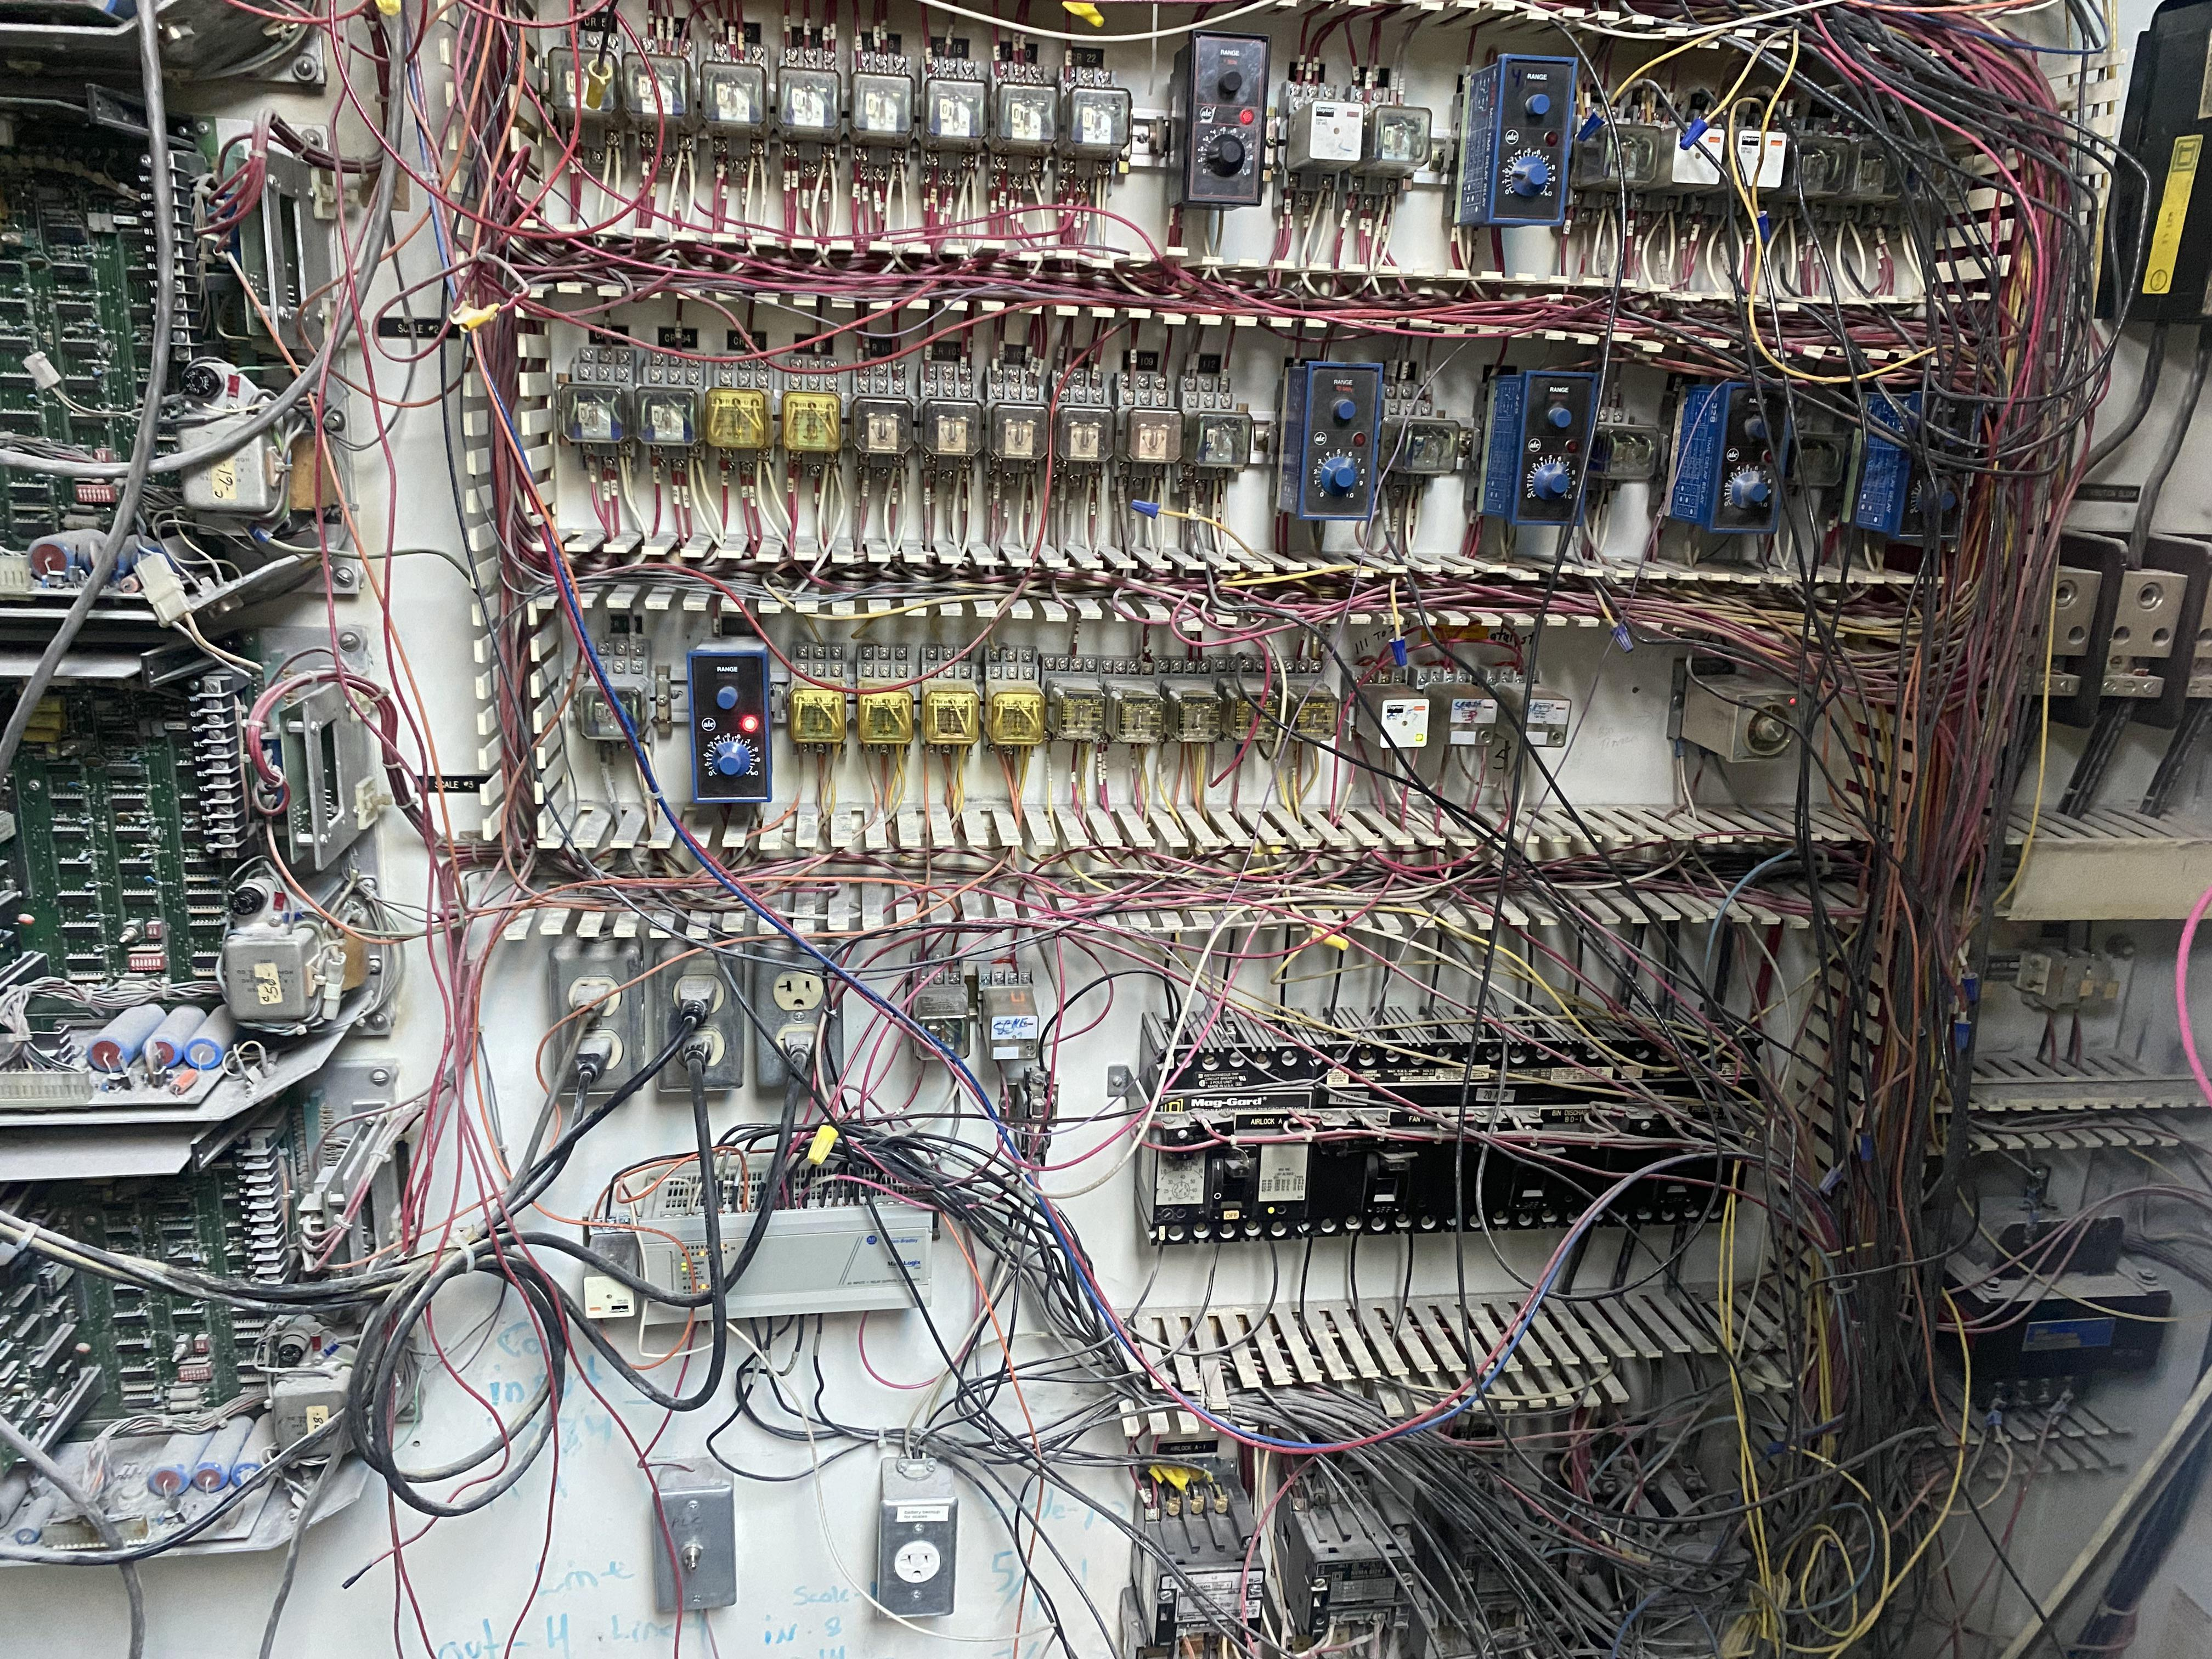
\includegraphics[
    width=\linewidth,
    height=0.39\textheight,
    keepaspectratio
]{figures/p01/rele.jpeg}

\vspace{0.25cm}

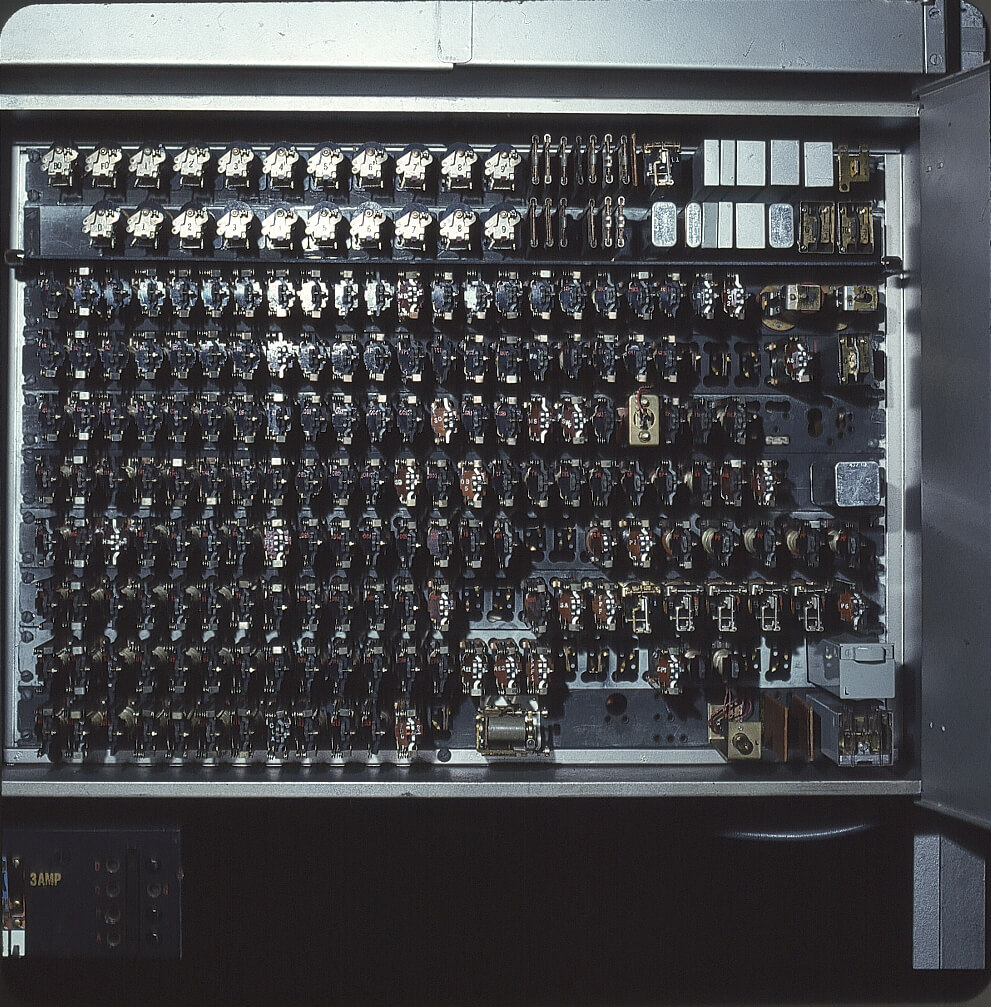
\includegraphics[
    width=\linewidth,
    height=0.39\textheight,
    keepaspectratio
]{figures/p01/rele2.jpg}

\vspace{0.12cm}

\end{columns}

\end{frame}

\begin{frame}{Colossus: špecializovaný elektronický výpočet}
\begin{columns}[T,onlytextwidth]
\column{0.47\textwidth}
\begin{itemize}
  \item 1943/1944: elektronický stroj pre kryptografickú analýzu.
  \item Ukázal, že rozsiahla logická úloha sa dá riešiť rýchlejšie elektronicky než mechanicky.
  \item Nebol to mikrokontrolér, ale ukazuje prechod od mechaniky k elektronickej logike.
\end{itemize}
\BlueBox{
    \faIcon{microchip}\hspace{0.5em}Základná myšlienka
}{
    Rýchlosť logiky začala byť určovaná elektronikou, nie pohybom mechanických kontaktov.
}
% ============================================================
% PRAVÝ STĹPEC – ŠTYRI OBRÁZKY
% ============================================================
\column{0.43\textwidth}

\centering
\vspace{0.10cm}

% Horný riadok
\begin{minipage}[t]{0.48\linewidth}
    \centering
    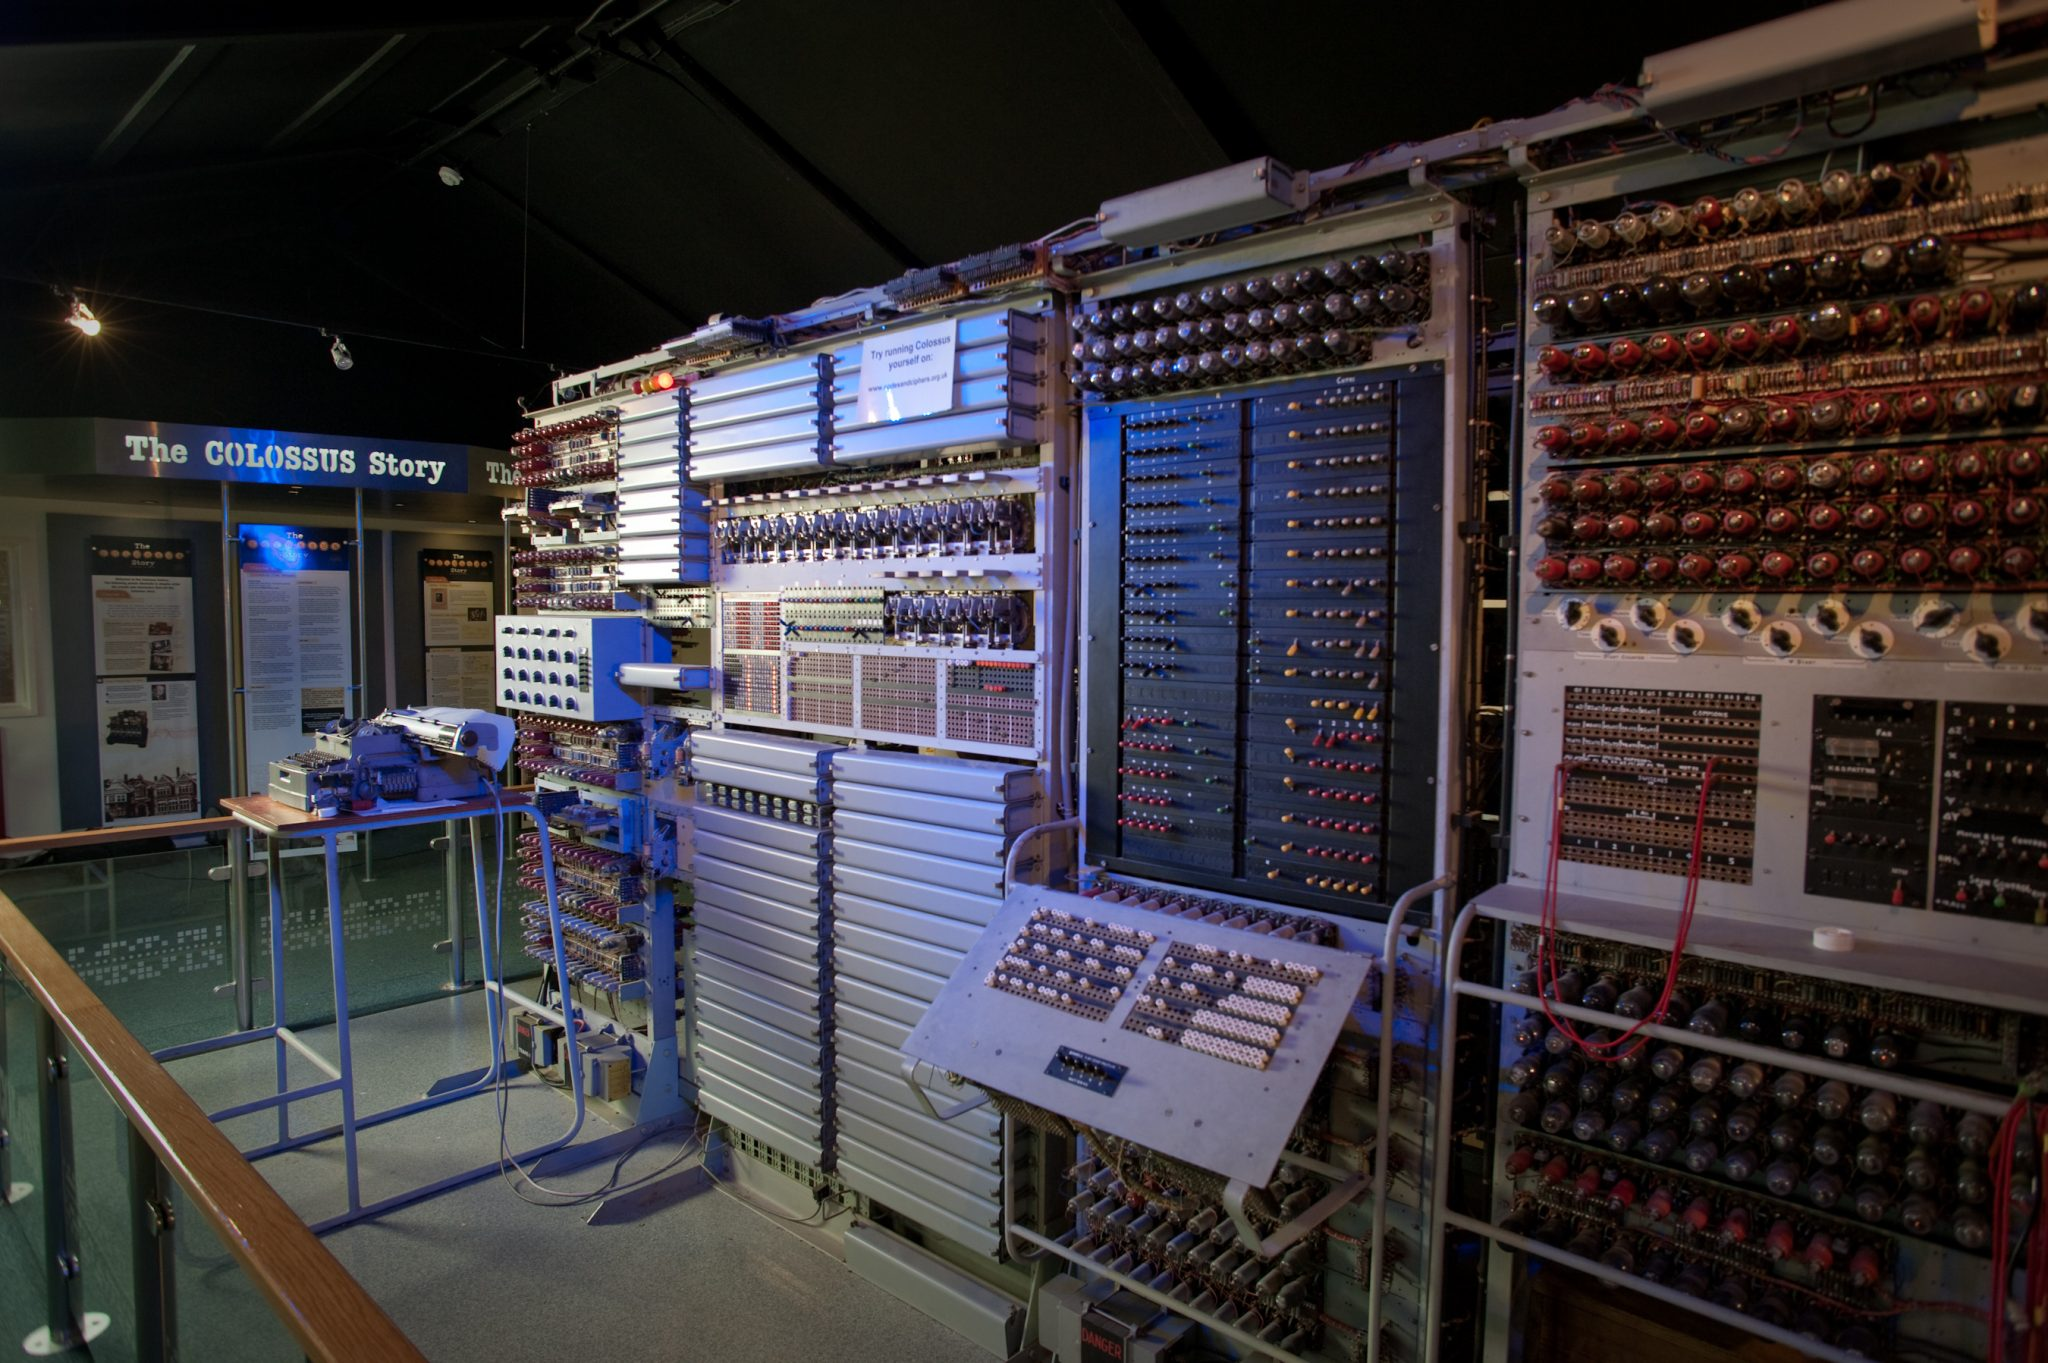
\includegraphics[
        width=\linewidth,
        height=0.35\textheight,
        keepaspectratio
    ]{figures/p01/colossus.jpg}
\end{minipage}
\hfill
\begin{minipage}[t]{0.48\linewidth}
    \centering
    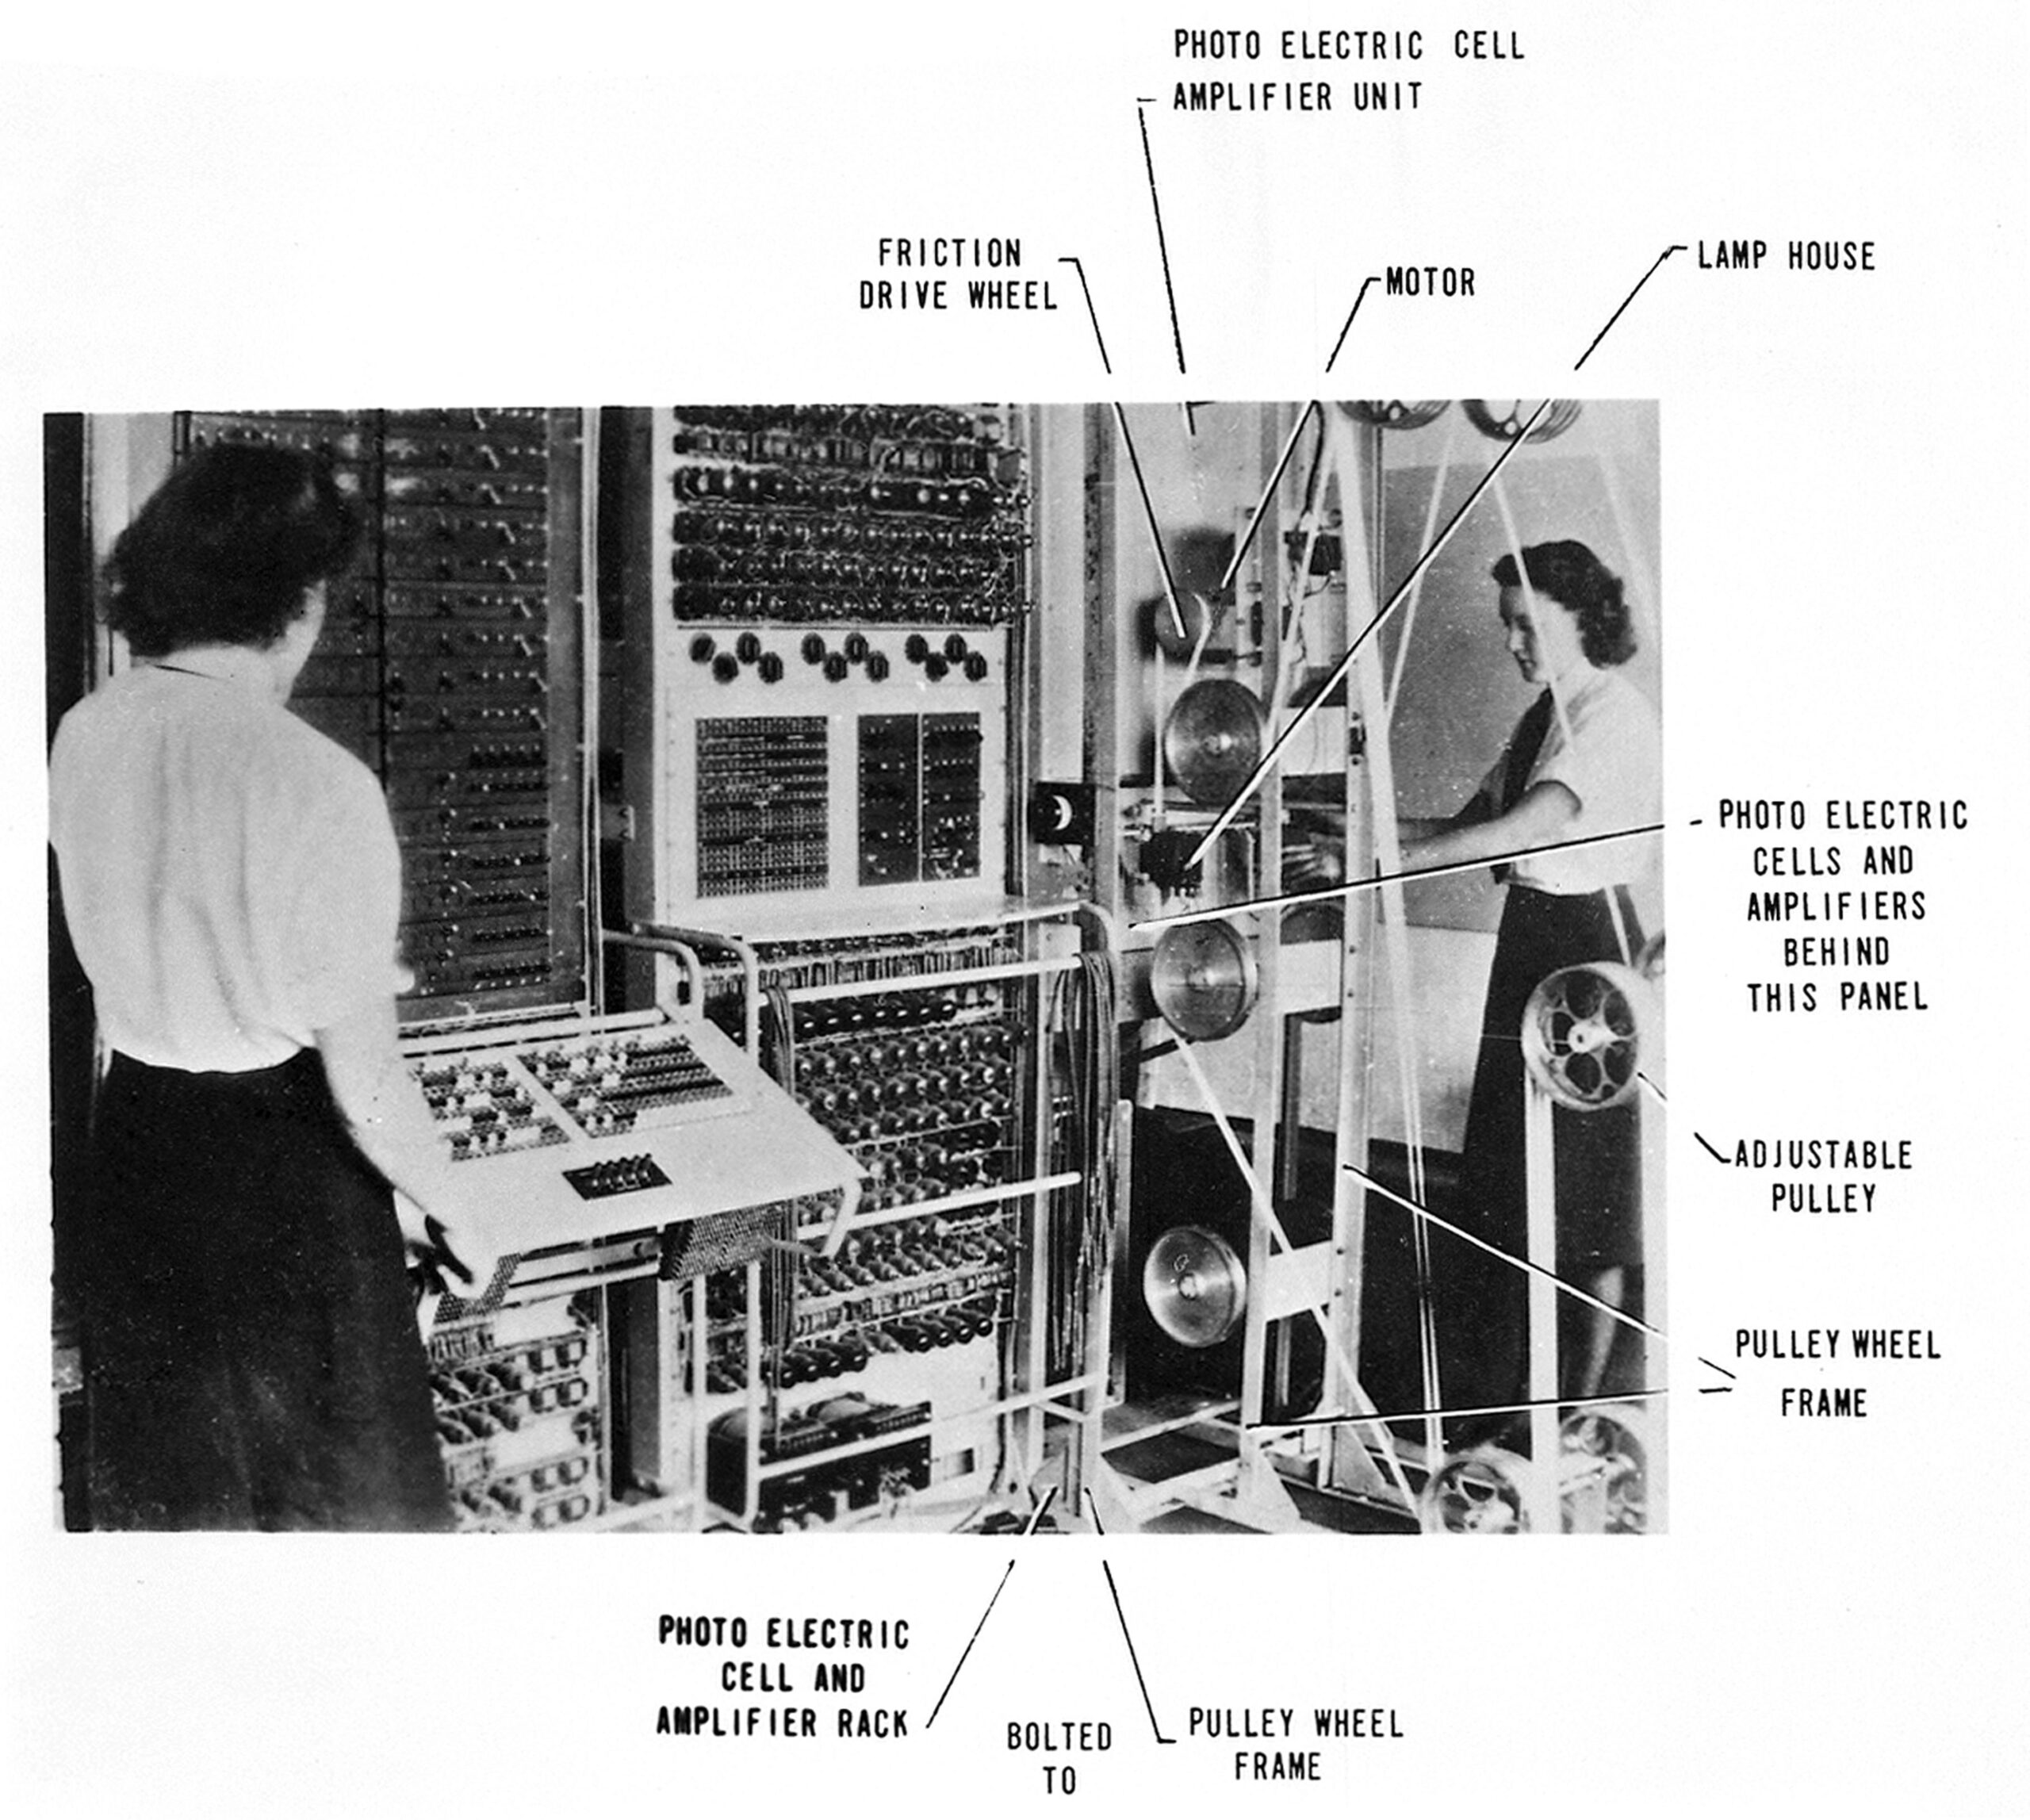
\includegraphics[
        width=\linewidth,
        height=0.35\textheight,
        keepaspectratio
    ]{figures/p01/colossus2.jpg}
\end{minipage}

\vspace{0.18cm}

% Dolný riadok
\begin{minipage}[t]{0.48\linewidth}
    \centering
    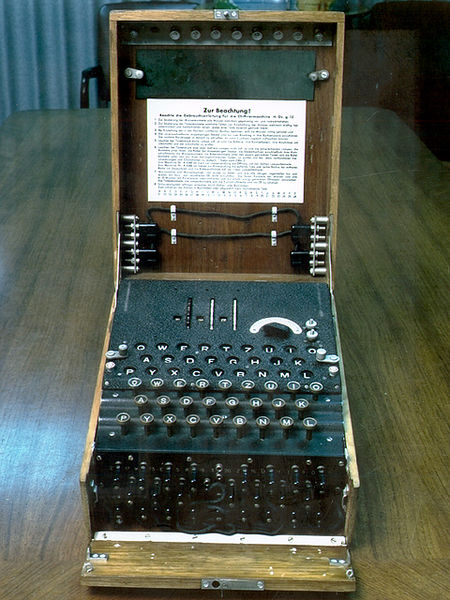
\includegraphics[
        width=\linewidth,
        height=0.35\textheight,
        keepaspectratio
    ]{figures/p01/enigma.jpg}
\end{minipage}
\hfill
\begin{minipage}[t]{0.48\linewidth}
    \centering
    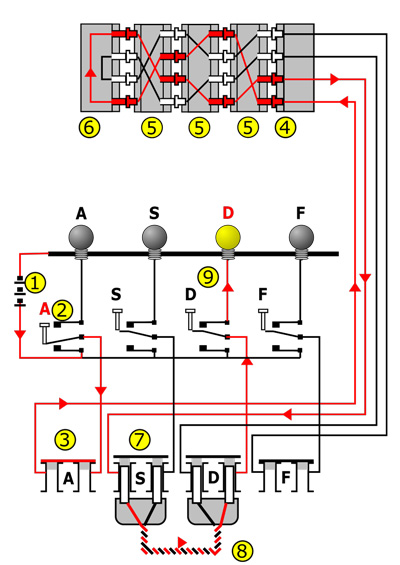
\includegraphics[
        width=\linewidth,
        height=0.35\textheight,
        keepaspectratio
    ]{figures/p01/enigma2.jpg}
\end{minipage}

\end{columns}
\end{frame}

\begin{frame}{ENIAC: elektromechanický počítač}
\begin{columns}[T,onlytextwidth]
\column{0.56\textwidth}
\begin{itemize}
  \item 1946: elektronický počítač založený na elektrónkach.
  \item Veľký výkon na svoju dobu, ale extrémne rozmery, spotreba a zložité programovanie.
  \item Programovanie často znamenalo prepájanie káblov a nastavovanie prepínačov.
  \item V r. 1948 upravený na čítanie z ROM: spomalenie výkonu 6-násobne, zmena dĺžky programovania z niekoľkých dní na hodiny
  \item Obsahoval: 21 501 elektróniek, 7200 kryštálových diód, 1500 relé, 70 000 rezistorov, 
     5 mil. ručne spájkovaných spojov, váha 30 t, rozmer 63 m2
\end{itemize}
\column{0.38\textwidth}
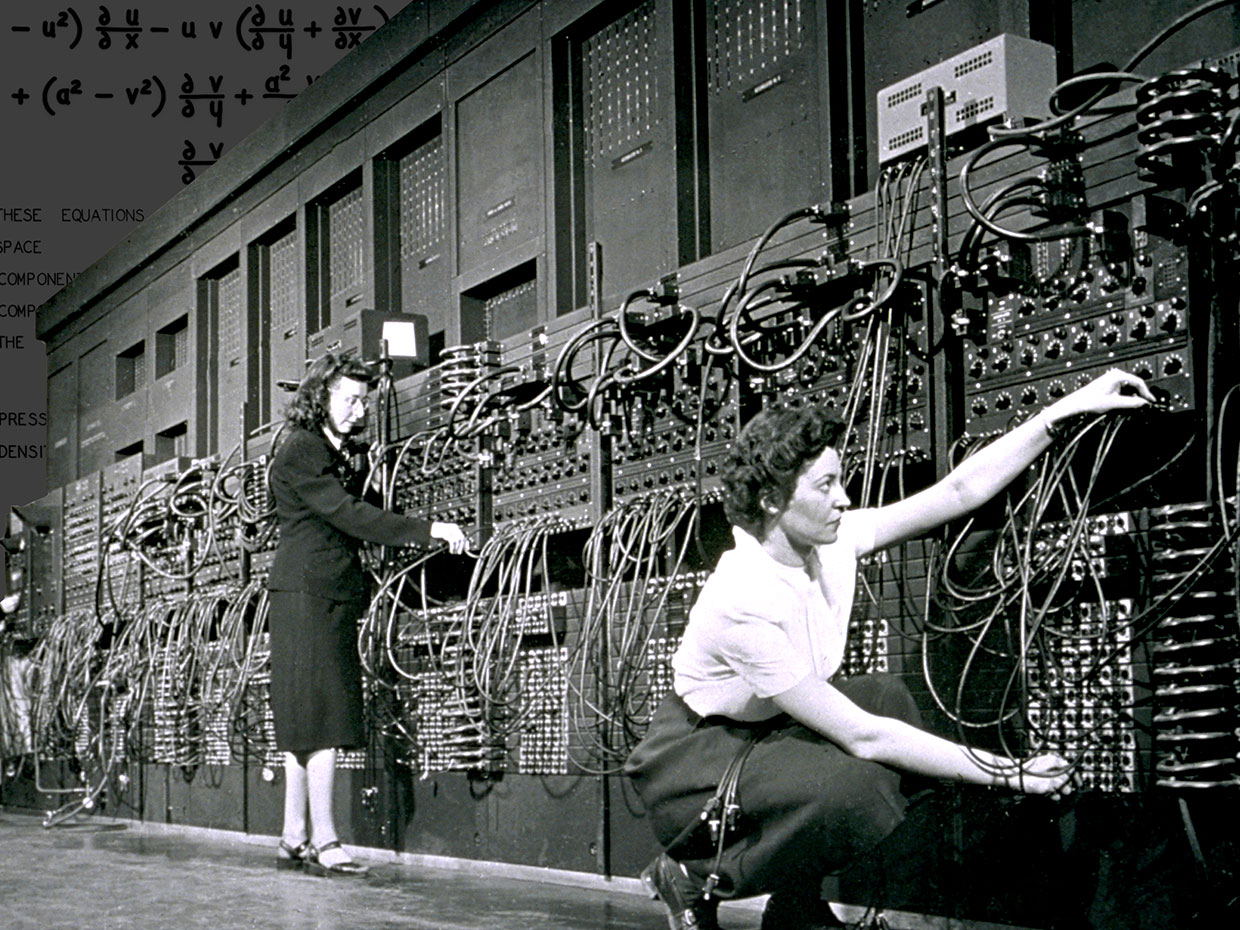
\includegraphics[width=\linewidth,height=5.4cm,keepaspectratio]{figures/p01/eniac.jpg}
\end{columns}
\end{frame}


\begin{frame}{Dôležitý historický problém: ako meniť funkciu stroja?}

\vspace{0.15cm}

\centering

\begin{tikzpicture}[
    stage/.style={
        draw=MainBlue,
        rounded corners=3pt,
        text width=3.25cm,
        minimum height=3.15cm,
        inner xsep=7pt,
        inner ysep=9pt,
        align=center
    }
]

% ============================================================
% PEVNÉ ZAPOJENIE
% ============================================================
\node[
    stage,
    fill=TUKEgray
] (wired) at (0,0)
{%
    {\large\bfseries Pevné zapojenie}

    \vspace{0.35cm}

    {\small
    Funkcia zariadenia je určená fyzickým zapojením obvodov.
    }

    \vfill

    {\color{MainBlue}\small\bfseries
    Zmena = prestavba hardvéru
    }
};

% ============================================================
% PREPÍNAČE A KÁBLE
% ============================================================
\node[
    stage,
    fill=LightBlue
] (panel) at (4.45,0)
{%
    {\large\bfseries Prepínače a káble}

    \vspace{0.35cm}

    {\small
    Funkcia stroja sa mení nastavením prepínačov a prepojením vodičov.
    }

    \vfill

    {\color{MainBlue}\small\bfseries
    Zmena = nové prepojenie
    }
};

% ============================================================
% PROGRAM V PAMÄTI
% ============================================================
\node[
    stage,
    fill=MainBlue,
    text=white
] (program) at (8.90,0)
{%
    {\large\bfseries Program v pamäti}

    \vspace{0.35cm}

    {\small
    Funkciu stroja určujú inštrukcie uložené v pamäti.
    }

    \vfill

    {\color{white}\small\bfseries
    Zmena = nový program
    }
};

% ============================================================
% ŠÍPKY
% ============================================================
\draw[
    ->,
    MainBlue,
    line width=1.1pt
] (wired.east) -- (panel.west);

\draw[
    ->,
    MainBlue,
    line width=1.1pt
] (panel.east) -- (program.west);

\end{tikzpicture}

% \vspace{0.05cm}

\BlueBox{
    \faIcon[regular]{lightbulb}\hspace{0.6em}Kľúčový posun
}{
    \parbox[c][1.25cm][c]{\linewidth}{
        Zavedením programu uloženého v pamäti sa oddelila funkcia stroja
        od jeho fyzického zapojenia. Správanie systému bolo možné meniť
        úpravou programu bez prestavby hardvéru.
    }
}

\end{frame}

\begin{frame}{Tranzistor: základ dnešnej číslicovej techniky}
\begin{columns}[T,onlytextwidth]
\column{0.47\textwidth}
\begin{itemize}
  \item 1947: tranzistor ako polovodičový spínací a zosilňovací prvok.
  \item Oproti elektrónkam priniesol menšie rozmery, nižšiu spotrebu a vyššiu spoľahlivosť.
  \item Umožnil vytvoriť integrované obvody a neskôr mikroprocesory.
\end{itemize}
\begin{alertblock}{Pre študenta}
Každý bit v registri mikrokontroléra je nakoniec realizovaný fyzikálnou štruktúrou z tranzistorov.
\end{alertblock}
\column{0.48\textwidth}

\includegraphics[width=\linewidth,height=4.8cm,keepaspectratio]{transistor_photos.png}
\end{columns}
\end{frame}

\begin{frame}{Integrovaný obvod: logika sa zmenšuje a zlacňuje}
\begin{columns}[T,onlytextwidth]
\column{0.52\textwidth}
\begin{itemize}
  \item Integrácia znamená, že viaceré tranzistory a vodiče sú vytvorené na jednom čipe.
  \item Čím viac logiky je na čipe, tým menej externých spojov a tým vyššia spoľahlivosť.
  \item Základná otázka sa zmenila: koľko funkcie dokážeme dať do jedného obvodu?
\end{itemize}
\column{0.43\textwidth}
\begin{tikzpicture}[x=1cm,y=1cm,scale=0.74,transform shape]
\node[draw=MainBlue,fill=TUKEgray,rounded corners=2pt,minimum width=3.0cm,minimum height=0.9cm] (g1) at (0,2.7) {hradlá};
\node[draw=MainBlue,fill=TUKEgray,rounded corners=2pt,minimum width=3.0cm,minimum height=0.9cm] (g2) at (0,1.5) {registre};
\node[draw=MainBlue,fill=TUKEgray,rounded corners=2pt,minimum width=3.0cm,minimum height=0.9cm] (g3) at (0,0.3) {radič};
\node[draw=MainBlue,fill=MainBlue,text=white,rounded corners=2pt,minimum width=3.0cm,minimum height=3.3cm,align=center] (chip) at (4.4,1.5) {integrovaný\\obvod};
\draw[->,MainBlue,line width=1pt] (g1) -- (chip.west);
\draw[->,MainBlue,line width=1pt] (g2) -- (chip.west);
\draw[->,MainBlue,line width=1pt] (g3) -- (chip.west);
\end{tikzpicture}
\end{columns}
\end{frame}

\begin{frame}{Moorov zákon: prečo sa výpočtová technika tak zrýchlila}
\begin{columns}[T,onlytextwidth]
\column{0.43\textwidth}
\begin{itemize}
  \item Rast počtu tranzistorov umožnil vyšší výkon a nové funkcie.
  \item V mikroprocesoroch viedol k zložitejším CPU a väčším pamätiam.
  \item V embedded systémoch však nie je cieľom iba výkon: dôležitá je cena, spotreba, spoľahlivosť a periférie.
\end{itemize}
\column{0.52\textwidth}

\includegraphics[width=\linewidth,height=5.1cm,keepaspectratio]{moore_graph.png}
\end{columns}
\end{frame}

\begin{frame}{Intel 4004: CPU na jednom čipe}
\begin{columns}[T,onlytextwidth]
\column{0.54\textwidth}
\begin{itemize}
  \item 1971: komerčný 4-bitový mikroprocesor.
  \item Približne 2300 tranzistorov, 16-pinové púzdro.
  \item Vznikol v kontexte kalkulačiek firmy Busicom.
  \item Dôležitý nie je iba výkon, ale nový princíp: procesor ako samostatný integrovaný obvod.
\end{itemize}
\column{0.41\textwidth}

\includegraphics[width=\linewidth,height=4.7cm,keepaspectratio]{intel4004_photos.png}
\end{columns}
\end{frame}

\begin{frame}{Intel 8008: 8-bitové spracovanie dát}
\begin{columns}[T,onlytextwidth]
\column{0.60\textwidth}
\begin{itemize}
  \item 1972: 8-bitový mikroprocesor.
  \item Prechod na 8 bitov uľahčil prácu so znakmi, bajtmi a všeobecnejšími dátami.
  \item Vyžadoval však externé obvody: pamäte, vstupno-výstupné rozhrania a podpornú logiku.
  \item Ešte stále nejde o mikrokontrolér, ale o CPU, okolo ktorého treba postaviť systém.
\end{itemize}
\column{0.34\textwidth}

\includegraphics[width=\linewidth,height=4.8cm,keepaspectratio]{intel8008_chip.png}
\end{columns}
\end{frame}

\begin{frame}{Intel 8080: mikroprocesor ako základ riadiaceho systému}
\begin{columns}[T,onlytextwidth]
\column{0.55\textwidth}
\begin{itemize}
  \item 1974: výrazne výkonnejší 8-bitový mikroprocesor.
  \item Používal sa v skorých mikropočítačoch a riadiacich aplikáciách.
  \item Ukázal, že mikroprocesor môže byť centrom všeobecného programovateľného systému.
  \item Pre embedded aplikácie však stále ostával problém veľkosti a počtu externých obvodov.
\end{itemize}
\column{0.40\textwidth}

\includegraphics[width=\linewidth,height=5.1cm,keepaspectratio]{intel8080_collage.png}
\end{columns}
\end{frame}

\begin{frame}{Z mikroprocesorového systému k mikrokontroléru}
\begin{center}
\begin{tikzpicture}[x=1cm,y=1cm]
\node[draw=MainBlue,fill=LightBlue,rounded corners=2pt,minimum width=2.5cm,minimum height=0.85cm] (cpu) at (0,2.3) {CPU};
\node[draw=MainBlue,fill=TUKEgray,rounded corners=2pt,minimum width=2.5cm,minimum height=0.85cm] (rom) at (3.2,3.2) {ROM / Flash};
\node[draw=MainBlue,fill=TUKEgray,rounded corners=2pt,minimum width=2.5cm,minimum height=0.85cm] (ram) at (3.2,2.0) {RAM};
\node[draw=MainBlue,fill=TUKEgray,rounded corners=2pt,minimum width=2.5cm,minimum height=0.85cm] (io) at (3.2,0.8) {I/O};
\node[draw=MainBlue,fill=MainBlue,text=white,rounded corners=2pt,minimum width=3.1cm,minimum height=3.0cm,align=center] (mcu) at (8.8,2.0) {CPU\\pamäť\\I/O\\periférie};
\draw[<->,MainBlue,line width=1pt] (cpu) -- (rom);
\draw[<->,MainBlue,line width=1pt] (cpu) -- (ram);
\draw[<->,MainBlue,line width=1pt] (cpu) -- (io);
\draw[->,MainBlue,line width=1.2pt] (5.1,2.0) -- node[above]{integrácia} (7.1,2.0);
\node[font=\small,align=center,text width=4.1cm] at (1.6,0.15) {mikroprocesorový systém z viacerých obvodov};
\node[font=\small,align=center,text width=4.0cm] at (8.8,0.15) {mikrokontrolér ako systém na jednom čipe};
\end{tikzpicture}
\end{center}
\end{frame}

\begin{frame}{TMS1000: CPU, pamäť a I/O na jednom čipe}
\begin{columns}[T,onlytextwidth]
\column{0.52\textwidth}
\begin{itemize}
  \item 1974: rodina mikrokontrolérov Texas Instruments TMS1000.
  \item 4-bitové jadro, ROM, RAM a vstupno-výstupné linky v jednom obvode.
  \item Vhodné pre lacné riadenie kalkulačiek, spotrebnej techniky a jednoduchých zariadení.
  \item Zlomová myšlienka: celý riadiaci systém môže byť integrovaný na jednom čipe.
\end{itemize}
\column{0.43\textwidth}

\includegraphics[width=\linewidth,height=5.1cm,keepaspectratio]{tms1000_collage.png}
\end{columns}
\end{frame}

\begin{frame}{Intel 8086: začiatok línie x86}
\begin{columns}[T,onlytextwidth]
\column{0.50\textwidth}
\begin{itemize}
  \item 1978: 16-bitový mikroprocesor.
  \item Dôležitý pre osobné počítače a neskorší vývoj architektúry x86.
  \item Ukazuje inú vetvu vývoja: všeobecné počítače smerovali k rastu výkonu, pamäte a operačným systémom.
  \item Mikrokontroléry smerovali k integrácii, nízkej cene a priamej práci s okolím.
\end{itemize}
\column{0.45\textwidth}

\includegraphics[width=\linewidth,height=5.1cm,keepaspectratio]{intel8086_collage.png}
\end{columns}
\end{frame}

\begin{frame}{Ďalšie míľniky: rozvetvenie vývoja}
\scriptsize
\begin{tabular}{p{0.14\textwidth}p{0.72\textwidth}}
\toprule
Rok & Význam pre mikroprocesorovú a embedded techniku \\
\midrule
1979 & Motorola 68000, Zilog Z8000 - výkonnejšie 16/32-bitové mikroprocesory \\
1980 & Intel 8051 - mimoriadne vplyvná 8-bitová mikrokontrolérová architektúra \\
1983 & TMS32010 - nástup digitálnych signálových procesorov DSP \\
1985 & Intel 80386 - 32-bitová x86 etapa \\
1986 & ARM - RISC architektúra s dôrazom na efektivitu \\
1990s & rozšírenie mikrokontrolérov v automobiloch, spotrebičoch a priemysle \\
2000s & masové embedded systémy, senzory, komunikácia, nízka spotreba \\
2010s+ & IoT, bezpečnosť, viacjadrové MCU, edge AI, hardvérová kryptografia \\
\bottomrule
\end{tabular}
\end{frame}

\begin{frame}{Intel 8051: klasická mikrokontrolérová škola}
\begin{itemize}
  \item 8051 je historicky veľmi významná 8-bitová mikrokontrolérová architektúra.
  \item Typická myšlienka: CPU, pamäť, porty, časovače a sériová komunikácia v jednom systéme.
  \item Mnohé princípy práce s registrami, portmi, prerušením a časovačmi sú podobné aj v AVR.
  \item Preto sa v embedded výučbe často nekladie dôraz na jednu značku čipu, ale na princíp periférií.
\end{itemize}
\begin{alertblock}{Poučenie}
Keď pochopíte jeden mikrokontrolér na úrovni registrov, ľahšie prejdete na ďalší.
\end{alertblock}
\end{frame}

\begin{frame}{ARM: RISC architektúra a nízka spotreba}
\begin{columns}[T,onlytextwidth]
\column{0.55\textwidth}
\begin{itemize}
  \item ARM ukazuje smer k výkonným, ale energeticky efektívnym embedded systémom.
  \item V praxi sa používa od jednoduchých mikrokontrolérov až po aplikačné procesory v mobilných zariadeniach.
  \item Dnešný embedded svet zahŕňa 8-bitové, 16-bitové aj 32-bitové architektúry.
\end{itemize}
\column{0.40\textwidth}
\BlueBox{Prečo teda AVR?}{
AVR je dostatočne jednoduchý na výučbu základov, ale pritom obsahuje reálne periférie používané v embedded praxi: GPIO, časovače, ADC, USART, SPI, TWI.
}
\end{columns}
\end{frame}

\begin{frame}{AVR: vhodná architektúra na výučbu registrov}
\begin{itemize}
  \item 8-bitové AVR mikrokontroléry majú prehľadnú architektúru a dobrú dokumentáciu.
  \item Majú oddelenú pamäť programu a dát, 32 všeobecných registrov a hardvérové periférie.
  \item Sú dostatočne jednoduché na pochopenie, ale nie sú didaktickou hračkou.
  \item ATmega328P je prakticky dostupný na doske Arduino UNO R3, čo znižuje problémy so zapojením.
\end{itemize}
\end{frame}

\begin{frame}{Historický záver}
\begin{center}
\begin{tikzpicture}[x=1cm,y=1cm]
\node[draw=MainBlue,fill=TUKEgray,rounded corners=2pt,minimum width=2.65cm,minimum height=0.8cm,align=center] (a) at (0,2.4) {\textbf{relé}\\\scriptsize pevné zapojenie};
\node[draw=MainBlue,fill=TUKEgray,rounded corners=2pt,minimum width=2.65cm,minimum height=0.8cm,align=center] (b) at (4.0,2.4) {\textbf{elektrónky}\\\scriptsize rýchla logika};
\node[draw=MainBlue,fill=TUKEgray,rounded corners=2pt,minimum width=2.65cm,minimum height=0.8cm,align=center] (c) at (8.0,2.4) {\textbf{tranzistor}\\\scriptsize miniaturizácia};
\node[draw=MainBlue,fill=LightBlue,rounded corners=2pt,minimum width=2.65cm,minimum height=0.8cm,align=center] (d) at (0,0.75) {\textbf{IC}\\\scriptsize integrácia};
\node[draw=MainBlue,fill=LightBlue,rounded corners=2pt,minimum width=2.65cm,minimum height=0.8cm,align=center] (e) at (4.0,0.75) {\textbf{CPU}\\\scriptsize mikroprocesor};
\node[draw=MainBlue,fill=MainBlue!18,rounded corners=2pt,minimum width=2.65cm,minimum height=0.8cm,align=center] (f) at (8.0,0.75) {\textbf{MCU}\\\scriptsize systém na čipe};
\draw[->,MainBlue,line width=1pt] (a) -- (b);
\draw[->,MainBlue,line width=1pt] (b) -- (c);
\draw[->,MainBlue,line width=1pt] (c.south) .. controls (8,-0.15) and (0,1.75) .. (d.north);
\draw[->,MainBlue,line width=1pt] (d) -- (e);
\draw[->,MainBlue,line width=1pt] (e) -- (f);
\end{tikzpicture}
\end{center}
\vspace{0.2cm}
\BlueBox{Zmysel tejto línie}{Mikrokontrolér vznikol, keď sa do jedného lacného a spoľahlivého obvodu integrovali výpočet, pamäť a priame rozhranie s okolím.}
\end{frame}
